\documentclass{ximera}

\author{Anna Davis} \title{MTH 240 Homework 3} 

\begin{document}

\begin{abstract}

\end{abstract}
\maketitle
 \textit{Certificate due: 2/3/2021 at 11:59 p.m.}
 
 \begin{problem}\label{prob:240hom3prob4}
 Average velocity is equal to the ...
 \begin{multipleChoice}  
\choice{slope of the tangent line to the graph of the position function}  
\choice{value of the position function at the point of tangency}  
\choice{value of the position function at 0}  
\choice[correct]{slope of the secant line to the graph of the position function}  
\end{multipleChoice}  
 \end{problem}
 
 \begin{problem}\label{prob:240hom3prob5}
 Instantaneous velocity is equal to the ...
 \begin{multipleChoice}  
\choice[correct]{slope of the tangent line to the graph of the position function}  
\choice{value of the position function at the point of tangency}  
\choice{value of the position function at 0}  
\choice{slope of the secant line to the graph of the position function}  
\end{multipleChoice}  
 \end{problem}
 
 \begin{problem}\label{prob:240hom3prob1}
 Suppose the height of a projectile fired upward is given by $$h(t)=-16t^2+48t+100$$
 \begin{enumerate}
     \item What is the initial height of the projectile?
     $$h_0=\answer{100}\mbox{ feet}$$
     \item When does the projectile reach its maximum height?
     $$\answer{1.5}\mbox{ sec}$$
     \item What is the maximum height?
     $$\answer{136}\mbox{ feet}$$
     \item When does the projectile hit the ground? (Round your answer to three decimal places.)
     $$t=\answer{4.415}\mbox{ sec}$$
 \end{enumerate}
 
In the graph below, manipulate the slider for $t_1$ to get various points on the position curve and answer the questions.

\begin{center}  
\desmos{udy4kct6jv}{800}{600}  
\end{center}

\begin{enumerate}
    \item Average velocity on the interval $0\leq t\leq 1$ is $\answer{32}$ feet per second.
    \item Average velocity on the interval $0\leq t\leq 1.5$ is $\answer{24}$ feet per second.
    \item Average velocity on the interval $0\leq t\leq 4$ is $\answer{-16}$ feet per second.
\end{enumerate}
\end{problem}

 \begin{problem}\label{prob:240hom3prob6}
 The value of the derivative is the \wordChoice{\choice[correct]{slope of the tangent line}, \choice{slope of the secant line}}
 \end{problem}

 \begin{problem}\label{prob:240hom3prob2}
 The manipulative below shows the graph of $f$ together with a secant line joining $(2,f(2))$ with $(a,f(a))$.  Manipulate the slider below to move the point $(a,f(a))$.  The secant line is labeled with its slope.  Use this information to estimate $f'(2)$ to the nearest integer.
 $$f'(2)=\answer{1}$$
 \begin{center}  
\desmos{xehtq4bysn}{800}{600}  
\end{center}

 \end{problem}
 
 \begin{problem}\label{prob:240hom3prob3}
 The figure below shows the graph of function $f$ together with two tangent lines to the graph at $(0, -1)$ and $(1.5,2)$.
 \begin{image}
   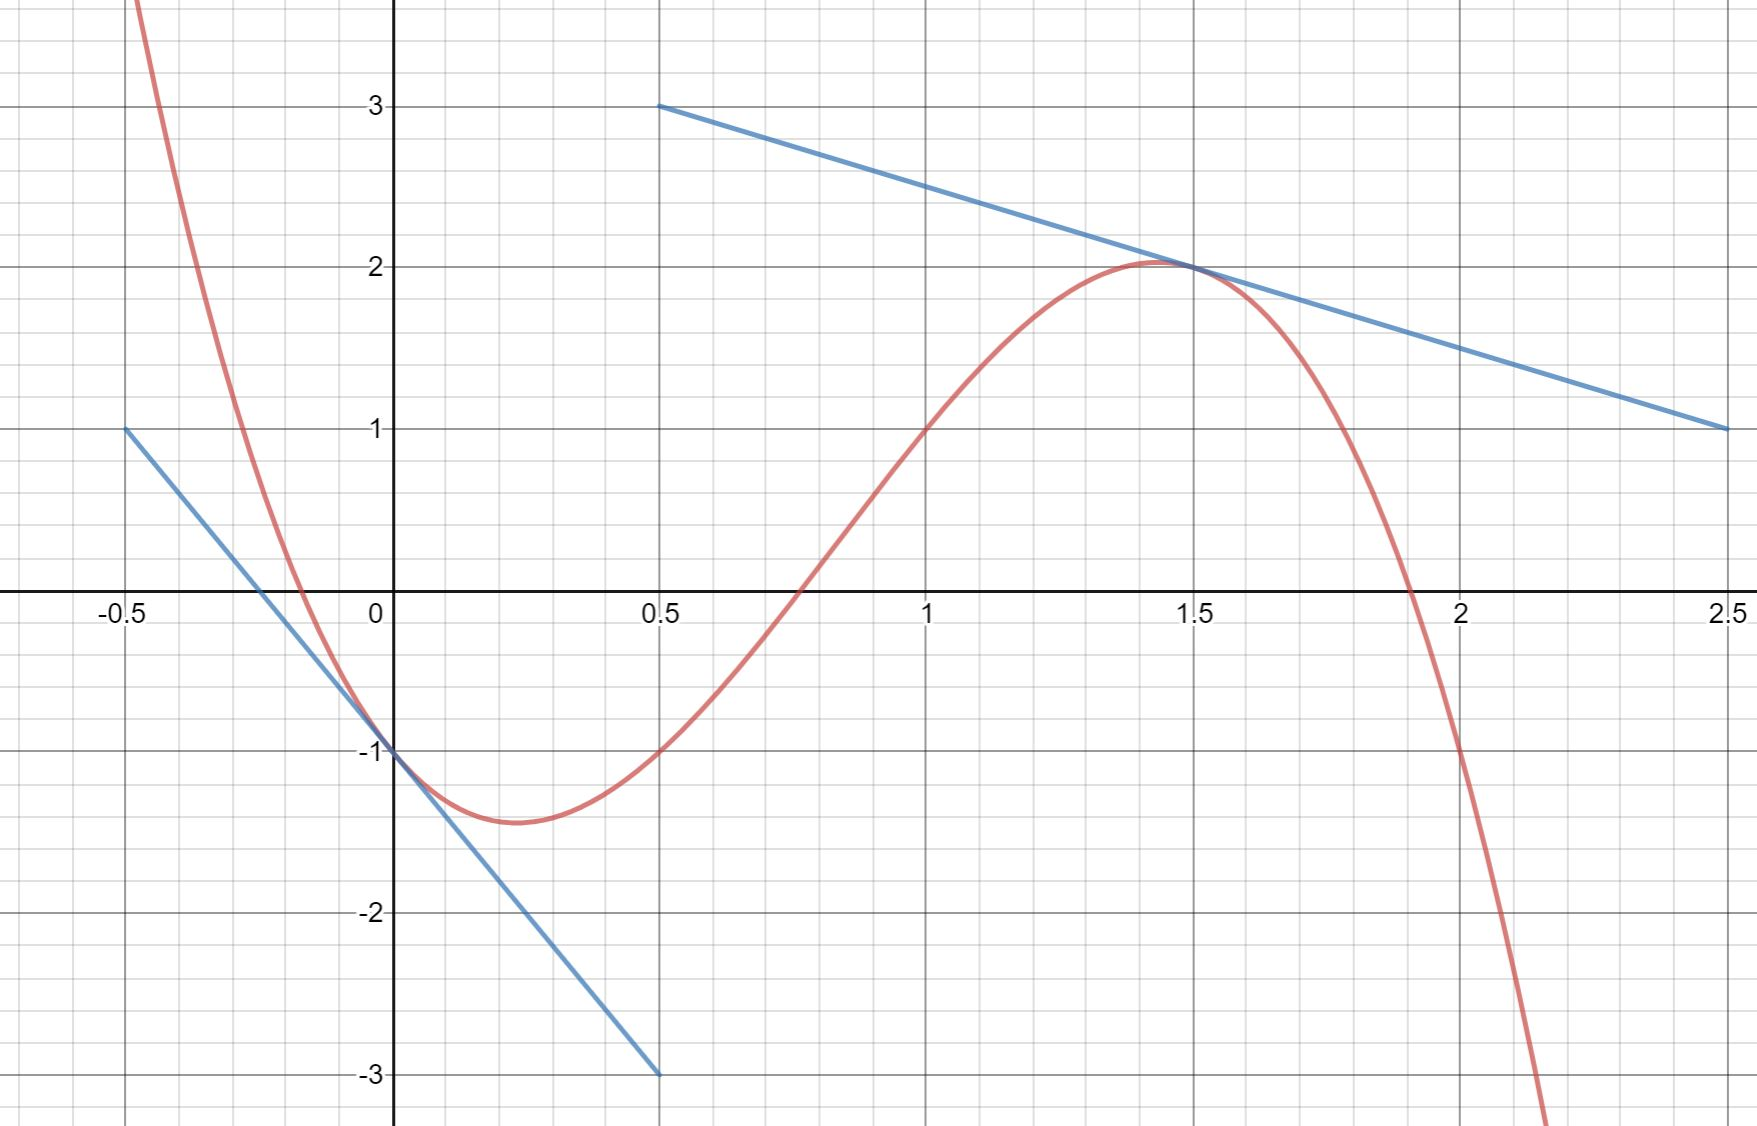
\includegraphics[height=1in]{240H3pic1.jpg}
 \end{image}
 Use the information in the graph to find the value of each derivative.
 $$f'(0)=\answer{-4}$$
 $$f'(1.5)=\answer{-1}$$
 
 \end{problem}
 
 \begin{image}  
  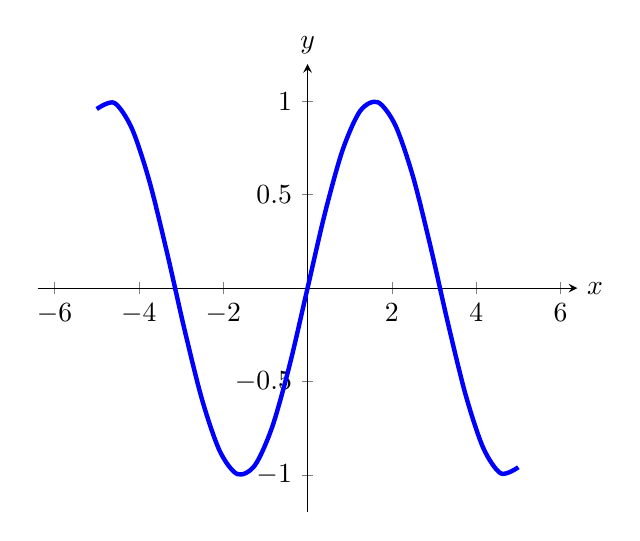
\begin{tikzpicture}  
    \begin{axis}[  
        xmin=-6.4,  
        xmax=6.4,  
        ymin=-1.2,  
        ymax=1.2,  
        axis lines=center,  
        xlabel=$x$,  
        ylabel=$y$,  
        every axis y label/.style={at=(current axis.above origin),anchor=south},  
        every axis x label/.style={at=(current axis.right of origin),anchor=west},  
      ]  
      \addplot [ultra thick, blue, smooth] {sin(deg(x))};  
    \end{axis}  
  \end{tikzpicture}  
\end{image}

\end{document} 